\documentclass[tikz,border=3pt]{standalone}
\usepackage[utf8]{inputenc}
\usepackage[T1]{fontenc}
\usepackage{lmodern}
\renewcommand{\familydefault}{\sfdefault}
\usepackage{sansmath}\sansmath
\usepackage{chemfig}
\usepackage{pgfplots}\pgfplotsset{compat=1.18,/pgf/number format/use comma,/pgf/number format/1000 sep={.}}
\usetikzlibrary{arrows.meta,calc,positioning,decorations.pathmorphing,patterns}
% paleta del sitio
\definecolor{nar}{HTML}{E8680C}\definecolor{narc}{HTML}{FFB35C}\definecolor{hielo}{HTML}{FFF3E8}
\definecolor{tinta}{HTML}{1D1D1F}\definecolor{gris}{HTML}{6E6E73}\definecolor{lila}{HTML}{7C5CF0}
\definecolor{azul}{HTML}{2F6FD6}\definecolor{menta}{HTML}{17A673}\definecolor{coral}{HTML}{E8342A}
\begin{document}
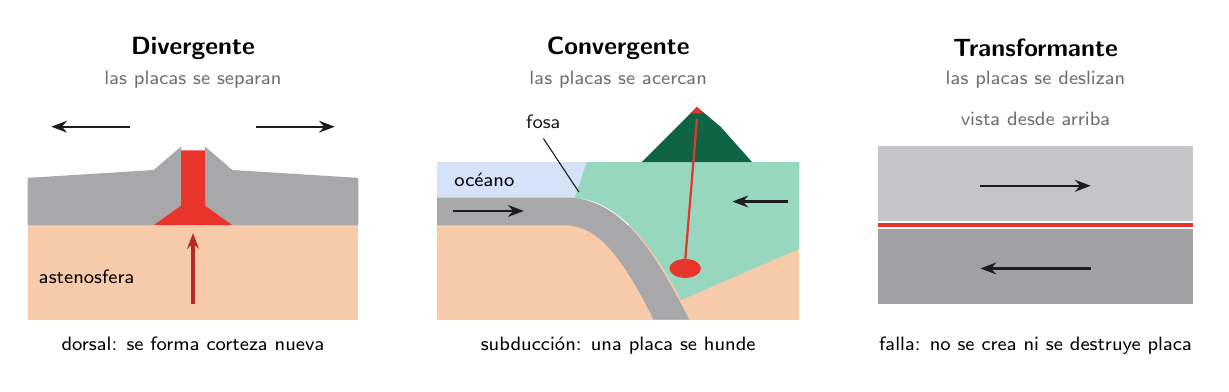
\begin{tikzpicture}[font=\footnotesize,>={Stealth[length=2mm]}]
% ---------- divergente
\begin{scope}
\node[font=\small\bfseries] at (2.1,3.45) {Divergente};
\node[font=\scriptsize,text=gris] at (2.1,3.05) {las placas se separan};
\fill[nar!35] (0,0) rectangle (4.2,1.2);
\fill[gris!60] (0,1.2) -- (0,1.8) -- (1.6,1.9) -- (1.95,2.2) -- (1.95,1.45) -- (1.6,1.2) -- cycle;
\fill[gris!60] (4.2,1.2) -- (4.2,1.8) -- (2.6,1.9) -- (2.25,2.2) -- (2.25,1.45) -- (2.6,1.2) -- cycle;
\fill[coral] (1.95,1.45) -- (1.95,2.15) -- (2.25,2.15) -- (2.25,1.45) -- (2.6,1.2) -- (1.6,1.2) -- cycle;
\draw[->,coral!80!black,very thick] (2.1,0.2) -- (2.1,1.1);
\draw[->,thick,tinta] (1.3,2.45) -- (0.3,2.45); \draw[->,thick,tinta] (2.9,2.45) -- (3.9,2.45);
\node[font=\scriptsize] at (0.75,0.55) {astenosfera};
\node[font=\scriptsize,anchor=north] at (2.1,-0.1) {dorsal: se forma corteza nueva};
\end{scope}
% ---------- convergente
\begin{scope}[xshift=5.2cm]
\node[font=\small\bfseries] at (2.3,3.45) {Convergente};
\node[font=\scriptsize,text=gris] at (2.3,3.05) {las placas se acercan};
\fill[nar!35] (0,0) rectangle (4.6,1.2);
\fill[azul!20] (0,1.2) rectangle (1.9,2.0);
\fill[gris!60] (0,1.2) -- (0,1.55) -- (1.7,1.55) .. controls (2.3,1.5) and (2.7,1.0) .. (3.2,0.0) -- (2.75,0.0) .. controls (2.3,0.9) and (2.0,1.2) .. (1.6,1.2) -- cycle;
\fill[menta!45] (1.9,2.0) -- (1.75,1.55) .. controls (2.3,1.5) and (2.7,1.0) .. (3.1,0.25) -- (4.6,0.9) -- (4.6,2.0) -- cycle;
\fill[menta!60!black] (2.6,2.0) -- (3.3,2.7) -- (3.6,2.45) -- (4.0,2.0) -- cycle;
\fill[coral] (3.22,2.62) -- (3.38,2.62) -- (3.3,2.7) -- cycle;
\fill[coral] (3.15,0.65) ellipse (0.2 and 0.12); \draw[coral,thick] (3.15,0.75) -- (3.3,2.55);
\draw[->,thick,tinta] (0.2,1.38) -- (1.1,1.38); \draw[->,thick,tinta] (4.45,1.5) -- (3.75,1.5);
\node[font=\scriptsize] at (0.6,1.78) {océano};
\draw[tinta] (1.8,1.62) -- (1.35,2.3) node[above,font=\scriptsize] {fosa};
\node[font=\scriptsize,anchor=north] at (2.3,-0.1) {subducción: una placa se hunde};
\end{scope}
% ---------- transformante (vista superior)
\begin{scope}[xshift=10.8cm]
\node[font=\small\bfseries] at (2.0,3.45) {Transformante};
\node[font=\scriptsize,text=gris] at (2.0,3.05) {las placas se deslizan};
\fill[gris!40] (0,1.25) rectangle (4,2.2);
\fill[gris!65] (0,0.2) rectangle (4,1.15);
\draw[coral,very thick] (0,1.2) -- (4,1.2);
\draw[->,thick,tinta] (1.3,1.7) -- (2.7,1.7); \draw[->,thick,tinta] (2.7,0.65) -- (1.3,0.65);
\node[font=\scriptsize,text=gris] at (2.0,2.55) {vista desde arriba};
\node[font=\scriptsize,anchor=north] at (2.0,-0.1) {falla: no se crea ni se destruye placa};
\end{scope}
\end{tikzpicture}
\end{document}
